\documentclass{standalone}

\begin{document}
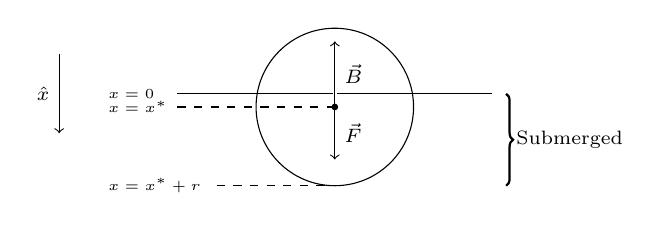
\begin{tikzpicture}
\usetikzlibrary{decorations.pathreplacing,angles,quotes}
\usetikzlibrary{shapes.geometric,shapes.misc}

    \draw (-3, 0) node[right] {\tiny $x = 0$} (-2, 0)  -- (2, 0);
    \draw (0, -1/6) circle (1);

    \draw[dashed] (-3, -1/6) node[right] {\tiny $x = x^*$}
        (-2, -1/6) -- (0, -1/6);

    \draw[dashed] (-3, -7/6) node[right] {\tiny $x = x^* + r$}
        (-1.5, -7/6) -- (0, -7/6);


    \draw[
        thick,
        decoration={brace,raise=5pt},
        decorate
    ] (2, 0) -- node[right=5pt] {\scriptsize Submerged}
      (2, -7/6);

    \draw[->] (0, -1/6) -- node[right] {\scriptsize $\vec{F}$} (0, -5/6);

    \draw[line width = 0.5mm, white, ->] (0, -1/6) -- (0, 4/6);
    \draw[->] (0, -1/6) -- node[right] {\scriptsize $\vec{B}$} (0, 4/6);

    \draw[fill = black] (0, -1/6) circle (1pt);

    \draw[->] (-3.5, 1/2) -- node[left] {\scriptsize $\hat x$} (-3.5, -1/2);

\end{tikzpicture}
\end{document}
